\chapter{Introduction}
\label{chapter:introduction}

\section{Motivation}
\label{section:motivation}

The Hash Code programming competition was a yearly event held by Google where
teams were challenged to solve a complex problem using any tools, resources, and
programming languages of their choice in just four hours. The problems were
typically inspired by issues arising in engineering and real-world situations,
such as vehicle routing, task scheduling, and Wi-Fi router placement.
Essentially, they were posed as ``open'' research problems for which there
exists a variety of solutions of different qualities. Notably, the great
majority of these are Combinatorial Optimization (CO) problems concerning the
search for the best solutions among a potentially large set of candidate
solutions. Thus the adoption of efficient search strategies that take the
available time budget into account is of utmost importance. Moreover, in the
context of the competition, the contestants must also read, understand the
problem, find a suitable representation, and write the code to solve it. As
such, not all of the available time can be spent in the solution optimization
stage.

A large number of optimization tools of different natures are available to
practitioners for solving CO problems. In particular, there are approaches that
are guaranteed to yield optimal solutions, although they are seldom appropriate
in a competition context due to their poor time performance on large problems,
such as the Hash Code challenges.

Albeit, for solving CO problems, a variety of algorithms exist that
typically offer a compromise between the runtime and quality of the solutions
found. Heuristics are a set of, often problem-specific, procedures that attempt
to quickly solve a problem and provide a helpful ``rule of thumb'' for
achieving reasonably good results, usually in a greedy fashion. A superset of
these algorithms are called meta-heuristics, and contrary to regular heuristics,
these are generic and can be applied to a broad range of problems. Natural
processes and phenomena, such as collective behavior, natural selection, and
some physical properties of materials, inspire several meta-heuristic search
processes making them flexible and adaptable, although more computationally
intensive than more conventional heuristics.

In the context of the Google Hash Code competition, competitors frequently make
use of greedy and other heuristic strategies tailored to the challenge. Moreover,
meta-heuristics in this situation are not as popular due to the time constraints
imposed by the competition format. At first glance, the majority of
optimization problems are structurally different from one other, which makes it
demanding to write general-purpose heuristic solvers that can be easily reused.
On the other hand, it might not be worth the effort spent in the implementation
of such solvers, particularly as the benefit of using a simple heuristic
strategy may outweigh the development and the running cost of meta-heuristic
solvers such as evolutionary algorithms.

Optimization algorithms, including meta-heuristics usually follow some strategy
that guides the procedure in the search for solutions. Some of the main
strategies are constructive search and local search. Constructive search
algorithms work by starting with an empty or partially complete solution  and
building a complete and feasible solution by iteratively adding components
based on the solution current state and the problem constraints. In contrast,
local search algorithms develop a given initial solution to the problem by
introducing small changes that aim to improve it to a good local optimum and
ideally a global one. A common usage of these strategies in competitions to
start with a constructive search stage, in order to find good solutions quickly
and then taking advantage of a local search strategy in an attempt to enhance
those solutions even further.

It is evident that algorithms or solvers that utilize these search strategies
are highly dependent on the specific problem they are trying to solve. The
solver plays a crucial role in the problem-solving process as it is responsible
for finding a solution. However, without a comprehensive model that can provide
the solver with relevant information about the problem, the solver's
effectiveness may be impaired.

\begin{figure}[h]
      \centering
      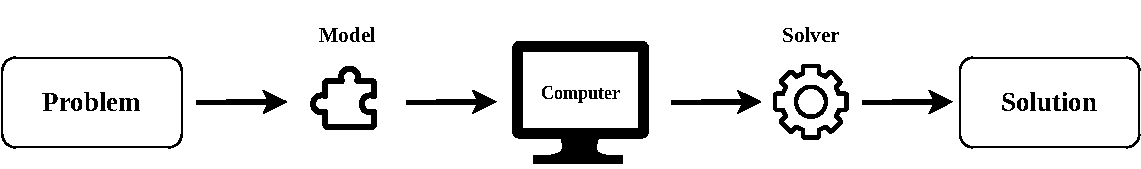
\includegraphics[width=\textwidth,keepaspectratio]{../assets/modelling/modelling.pdf}
      \caption{Modelling and Problem Solving}
      \label{fig:problem-solving}
\end{figure}

The model serves as a means of presenting the various aspects of the problem to
the computer, which will subsequently utilize a solver to find a
solution~\ref{fig:problem-solving}. When constructing a model, it is important
to include relevant features such as the representation of the problem and
solution, a description of how components can be added or removed from the
solution, and methods for evaluating the solution, calculating bounds, and
obtaining other heuristic information.

A good model should encode in it all the relevant information from the problem
and we must ask the right questions to obtain it, adhering to the philosophy that ---
``\textit{understanding the question is half the answer}''. Additionally, if a
model were to be built in a standardized way, this would allow the development of
a suite of generic and reusable (meta-heuristic) solvers that could find
solutions in a black-box fashion. This idea has already been explored to some
extent in previous work~\cite{outeiro2021application,vieira2009uma} and will be
further pursued.

It is worth noting that the modelling aspect in this field has often been
neglected by the community, which has been primarily focused on the development
of meta-heuristics algorithms (solvers). This discrepancy can be contrasted with
the mathematical perspective, where practitioners and researchers have
emphasized the importance of clearly separating the models and the algorithms
(solvers), and have placed a significant emphasis on the modelling perspective.
This gap highlights the importance of considering the modelling aspect in this
field.

Recently, there has also been growing interest within the community in the
development of optimization benchmark problems that are both relevant in
practical applications and amenable to theoretical analysis. The Hash Code
problems may be suitable candidates for this purpose, as they pose significant
challenges from a modelling perspective while also being easy to describable.
Furthermore, these problems have already been partially solved to some extent
in a competitive setting, and there is a wealth of empirical data available on
the best known solutions and seldomly the method used to obtain them. Overall,
these factors make the Hash Code problems an ideal testing ground for both
modelling and the evaluation of meta-heuristics.

\section{Contribution}
\label{section:contribution}

The main goal of this work is to develop and implement effective heuristic and
meta-heuristic approaches for solving Hash Code problems, with a particular
focus on the modelling aspect and the clear separation between solvers and
models. By doing so, we hope to develop more structured and efficient
problem-solving strategies that can effectively address a range of challenges.
Additionally, some effort will be made to address other key areas that are
crucial to the success of this work, namely:

\begin{itemize}
      \item Development and refinement of the frameworks that separate models from solvers
            currently materialized in an Application Programming Interface (API)
            designed only for constructive search~\cite{outeiro2021application}.
            The main goal is to optimize and ``fine-tune'' this API in order to improve its
            efficacy and utility, by using the Hash Code problems as benchmarks.

      \item Expansion of the aforementioned API to support local search strategies
            in a problem-independent manner. This will allow for its application to a wider
            range of problems and contexts.

      \item Implementation of a small set of general-purpose meta-heuristic solvers and utilities
            that can be used to not only generate and test solutions for the various
            Hash Code benchmark problems, but also to verify the correctness of the results.
\end{itemize}

Last but not least, the objective of this work is to engage in a critical
examination of the strengths and limitations of our adopted approach to problem
modelling and solver development. This discussion will be relevant to
meta-heuristic researchers, software developers, and practitioners alike. The
analysis will consider various performance dimensions, including the effort
required for problem modelling and solver development, the computational
efficiency of the implemented software, and the quality of the solutions
obtained.

\section{Research Questions}
\label{section:research-questions}

\section{Outline}
\label{section:outline}

The remainder of this document is structured as follows:

\begin{itemize}
      \item \textbf{Chapter~\ref{chapter:background}:} Provides some background
            on some essential aspects of optimization, search strategies,
            meta-heuristics, and modelling. Moreover, it presents the modelling
            frameworks and current state of the art of the API attempts that
            constitute the core fundamentals that~\cite{outeiro2021application}
            supports this work.

      \item \textbf{Chapter~\ref{chapter:preliminary-work}:}
            Gives some insight into the Google Hash Code competition and typical
            problems presented to contestants. Furthermore, it makes a brief
            categorization of all the problems from previous editions, with particular
            emphasis on the ones analyzed so far. Finally, it describes the modelling
            of the problems examined and the results obtained

            % \item \textbf{Chapter~\ref{chapter:conclusion}:} Presents a summary of the work
            %       completed and some observations about the next steps to be taken.

      \item \textbf{Chapter~\ref{chapter:conclusion}:} Presents a reflection on this work.
\end{itemize}

